\documentclass{article}
\usepackage[utf8]{inputenc}

\title{CS685 Data Mining - Assignment1}
\author{P J Leo Evenss(20111038) }
\date{\today}
\usepackage{graphicx}
\usepackage[section]{placeins}
\usepackage{hyperref}
\hypersetup{
    colorlinks=true,
    linkcolor=blue,
    filecolor=magenta,      
    urlcolor=cyan,
}

\urlstyle{same}
\begin{document}



\maketitle

\section{Introduction}
\vspace{0.5cm} 
\hspace{2cm} We live in a Covid-19 pandemic age, greatly affecting our health, mobility and behaviour. This short assignment gives us a brief outlook on the variations of covid confirmed cases across the country over the period of 15-Mar-2020 to 05-Sept-2020. \newline

\hspace{2cm} This report holds short conclusions and analysis drawn from the data extracted and preprocessed from the website \url{https://www.covid19india.org/}.



\section{Analysis}
\vspace{0.5cm} 
\hspace{2cm}The analysis of cases across months, districts are given as below:
\subsection{Overall Cases}
\vspace{0.5cm}
\hspace{2cm}As shown in the Figure 1, we observe, there has been a steady increase in the number of confirmed cases from the month of june. The graph indicates an overall increase of 78\% in august when compared to july. The ease of lockdown and other strict quarantine measures might have contributed to this spike of cases as compared to the months like april, may.    
\begin{figure}[htp] 
    \centering
    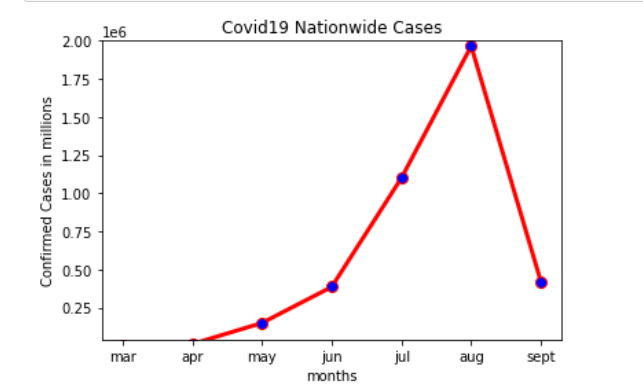
\includegraphics[width=10cm]{overallcases.png}
    \caption{The nationwide overall cases during  15th march - 5th sept} 
    \label{fig:graph}
\end{figure}
\FloatBarrier
\subsection{Delhi Cases}
\vspace{0.5cm}
\hspace{2cm}The Figure 2, shows the variations of cases in our country's capital state Delhi over the months. We notice the cases reached its spike in the month of june and has been steadily decreasing since then, giving a positive sign in the measures taken by the govt of India. The reason could also be that 60\% of the population of the Delhi has already been affected.




\begin{figure}[htp]
    \centering
    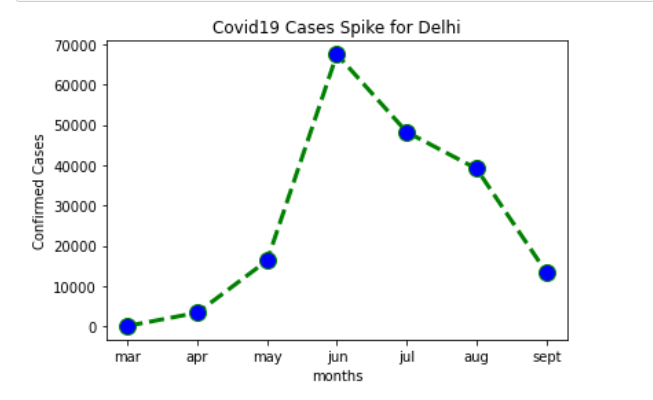
\includegraphics[width=10cm]{delhicases.png}
    \caption{The graph of cases in Delhi during 15th march - 5th sept}
    \label{fig:delhigraph}
\end{figure}
\FloatBarrier
\subsection{The Hotspots \& Coldspots}
\vspace{0.5cm}
\hspace{2cm} The Figure 3, shows the top 5 districts which are hotspots and coldspots and their cases respectively among all other districts in their state. We can observe that the districts like Bangalore , Chennai, Patna are projected as hotspots due to their dense population when compared to other districts in the state, and similarly Diu,Krishna fall under coldspots due to their relatively less population.\newline

\hspace{2cm} The hotspot and coldspots are calculated by taking into account the mean and standard deviation of all the other districts in the state and computing their respective z-scores.

\begin{figure}[htp]
    \centering
    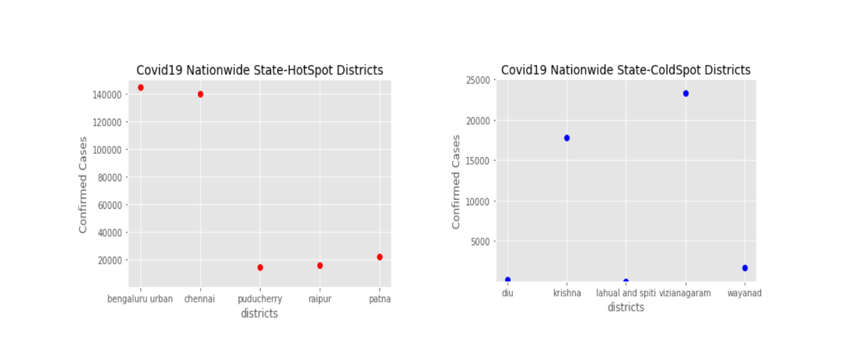
\includegraphics[width=15cm]{hotsptandcolspot.png}
    \caption{The graph of top 5 hotspot and coldspot districts in the states}
    \label{fig:hotspot}
\end{figure}
\FloatBarrier

\section{Conclusion}
\vspace{0.5cm}
\hspace{2cm} We thus notice the increase in the covid cases in several districts per week, month and their resulting central tendency and variations with respect to its neighbouring districts from the results of the assignment.\newline

\hspace{2cm}We can extend the above results in predicting the time period on which the cases reach the peak value and also when the covid pandemic might subside. Such analysis are being done by  competitive data scientists all over the globe to bring a ray of hope amidst the pandemic times. We have replicated a tiny piece of such data preprocessing in this assignment


\end{document}
